\chapter{Bundle Adjustment}

Bundle adjustment is the process of simultaneously adjusting the
properties of multiple cameras and the 3D locations of the objects
they see, to minimize the error between the estimated forward
projection of the 3D objects and their measured location in the captured
images. 

\begin{figure}[htp]
  \begin{center}
  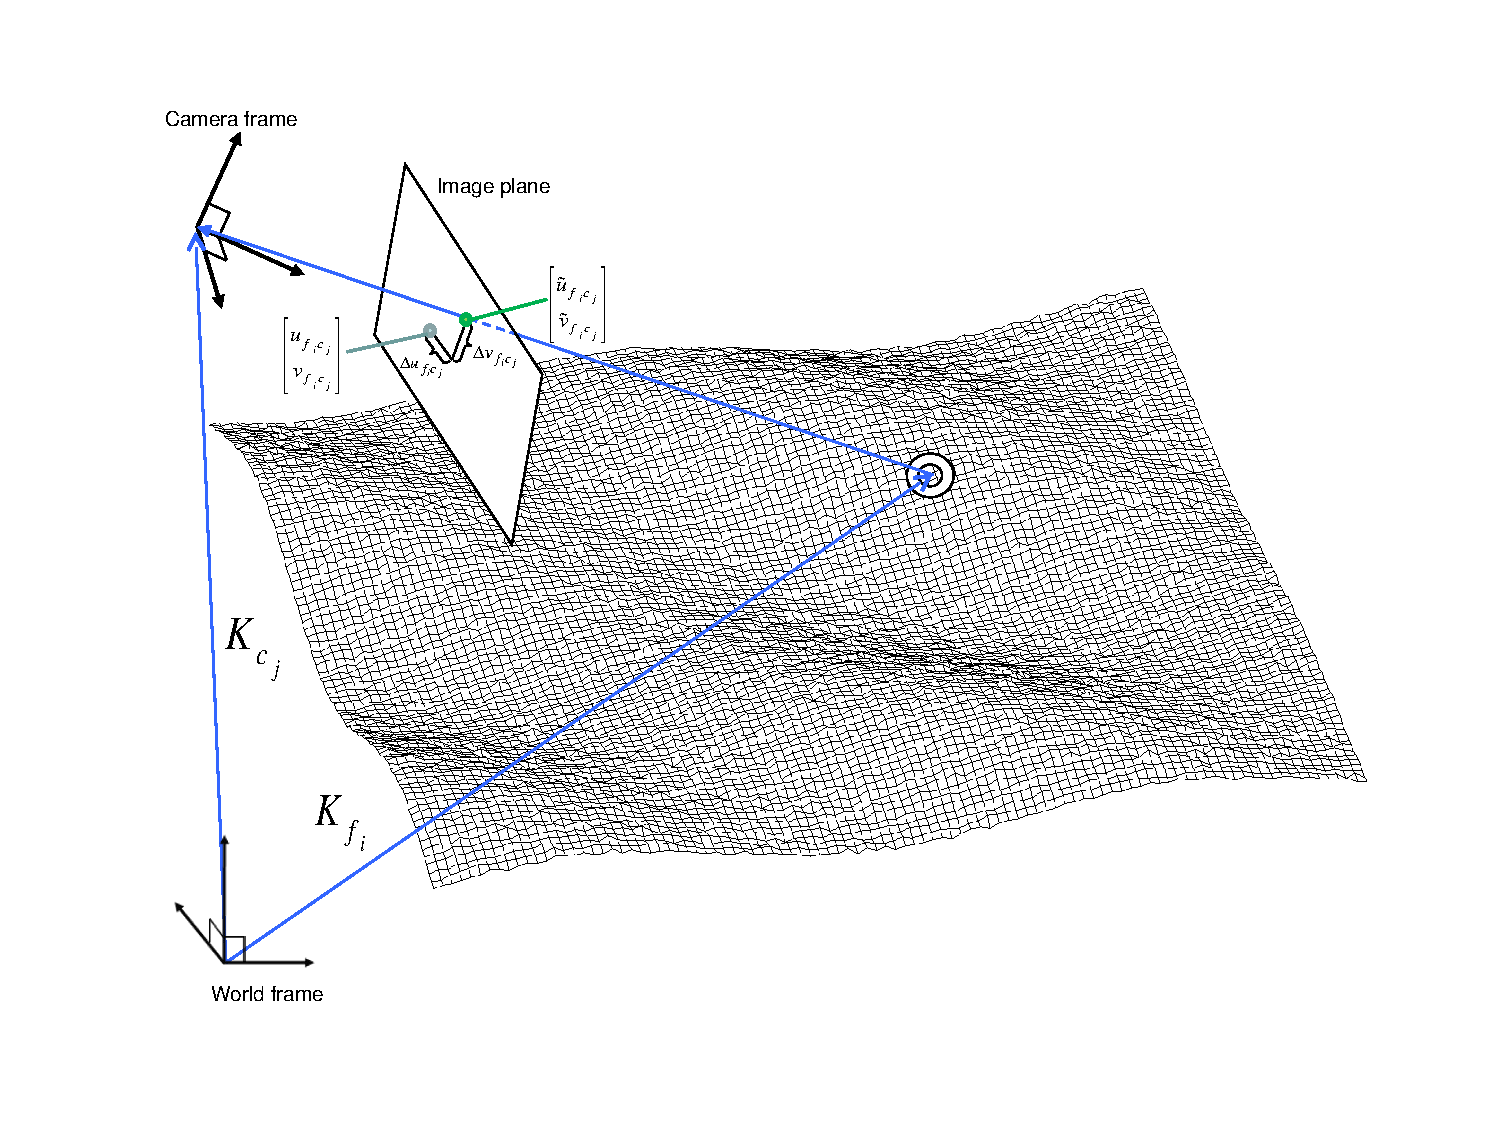
\includegraphics[trim=20mm 20mm 20mm 15mm,clip,width=6in]{images/ba_feature_observation.pdf}
  \end{center}
  \caption{ A feature observation in Bundle Adjustment. \cite{moore09} }
  \label{fig:ba_feature}
\end{figure}

This has application as an optional step between the capture
of images and the creation of DEMs. There is always an amount of error
with the recorded position and orientation of cameras and Bundle
Adjustment can be used to refine these measurements. This will allow
DEMs from multiple cameras to align better with one another. Bundle
Adjustment can also take advantage of Ground Control Points (GCPs),
which are accurately measured 3D locations on the surface of the DEM. GCPs
can be used to improve the alignment of the DEMs or align the new DEM
to a past data product. Finally, even though Bundle Adjustment
calculates the location of the 3D objects it views, only the final
properties of cameras are recorded in the Ames Stereo Pipeline. Those
properties are loaded into \texttt{stereo} which will then use it's own
method for triangulation.

\subsection{A deeper understanding}

Bundle Adjustment in Ames Stereo Pipeline revolves around the
Levenberg-Marquardt Algorithm (LMA) which is a method for minimizing a
function. In the case of Bundle Adjustment, the error $\epsilon$ is
the pixel difference between an objects location in an image,
$[u_{f},v_{f}]$, and it's forward projection through the camera,
$[\tilde{u}_{f},\tilde{v}_{f}]$. The goal is to solve for an update to
the parameters of the cameras and point positions, apply them, and
then repeat until the update supplied by LMA goes to zero. The
equation for LMA is below:

\begin{equation}
\mbox{\boldmath$\delta$} = \frac{\mbox{\boldmath$J^T\epsilon$}}{\bf{J^TJ}+\lambda\bf{I}}
\label{eqn: Levenberg-Marquardt Algorithm}
\end{equation}

LMA is a hybrid of two minimization techniques, gauss-newton and
gradient decent. Where the control between these two methods is the
parameter $\lambda$ which will change in value during the process of
Bundle Adjustment. A high value of $\lambda$ forces LMA to act like
gradient decent, and is what will happen at the beginning of bundle
adjustment when the camera parameters are far away from their final
solution. A low value of $\lambda$ drives LMA into the gauss-newton
method; at which it will take small steps in updating the camera
values. When Bundle Adjustment is almost finished and is close to the
solution, it will lower $\lambda$.

Since Bundle Adjustment is an iterative method, it would be happy to
keep processing new updates to camera parameters all day. To avoid
this, there are several shut-off conditions. The first is when the
update {\boldmath$\delta$} becomes insignificantly small. The second
is when the error measurement, {\boldmath$\epsilon$}, becomes
insignificantly small. Both of these conditions' thresholds are
defined within the bundle adjuster's code and is not allowed for the
user to change. The final shut off condition is when the number of
iterations becomes too large. It is important to understand that when
this shut off condition happens, bundle adjustment has not finished
refining the parameters of the cameras but they are a step closer to
the solution. The maximum number of iterations is changeable by the
user so they can decide how much time they're willing to dedicate to
the correction of the data. The number of iterations Bundle Adjustment
takes to converge on the solution can be anywhere between 20
iterations to several hundred.

If you are interested in more information on the math of Bundle
Adjustment and the arrangement of the problem, we recommend reading
Appendix 6 in the {\em Multiple View Geometry} \cite{hartley04}.
For more information on why LMA is used instead of the many other
optimization algorithms, try reading {\em Bundle Adjustment – A Modern
Synthesis} \cite{triggs00}.

\section{ISIS Adjust}

The \texttt{isis\_adjust} program is an application designed to
perform bundle adjustment on the cameras supported by USGS's
ISIS3. \texttt{isis\_adjust} is special in that it does not
discriminate based on camera type. It can perform bundle adjustment on
line-scan imagers (such as MOC and Apollo's Panoramic Camera) just as
well as it can on traditional frame cameras (such as Apollo Metric
Camera). Theoretically it should also work fine with push-frame
imagers (i.e. video), though this is untested.

\texttt{isis\_adjust} works by first converting all pixel measurements
in an images to measurements defined on the ideal focal
plane using millimeters and the ephemeris time (ET). The ET is the
absolute second at which that pixel measurement was recorded on the camera. 
For a frame camera, the ET won't change for the for
any of the measurements on the image. For anything more exotic, it is
a different story. On a MOC image between the top and bottom line;
about 5 seconds could have passed.

\begin{wrapfigure}{r}{0.3\textwidth}
\vspace{-30pt}
\begin{center}
  \definecolor{lgray}{gray}{0.95}
  \fcolorbox{black}{lgray}{\begin{minipage}{0.29\textwidth} 

      \emph{Note from Author:} \\ Currently \texttt{isis\_adjust}
      lacks a proper way to support arbitrary defined correction
      functions. For the time being, \texttt{isis\_adjust} has been
      hard-coded to perform only zero order corrections (i.e. scalar
      offsets). (03/11/09)

  \end{minipage}}
\end{center}
\vspace{-30pt}
\end{wrapfigure}

When \texttt{isis\_adjust} calculates the partial derivatives of the
forward projection of a point, it will use an ideal pinhole camera
model. The properties of the ideal pinhole camera are defined as
properties of the subject camera at the specificed ET for the current
measure plus the correction function $f(t)$ that \texttt{isis\_adjust} is
solving for. $f(t)$ can be almost any function of ET, the only limit is the
number parameters in the equations. Some initial work hints that
anything greater than a $2^{nd}$ order polynomial becomes an ill-posed
problem.

\subsection{Options}

The following is a listing and explanation of the command line options
that can be fed to \texttt{isis\_adjust} from the terminal.

\begin{verbatim}
--cnet, -c [control network file]
\end{verbatim}

\emph{Optional.} Feeding this option will force ISIS Adjust to use an
already built control network. This control network can either be in
the ISIS style format or the binary Vision Workbench style. If not
fed, ISIS Adjust will look for match files in current operating
directory with names similar to the input images to build it's control
network from. If \texttt{isis\_adjust} creates it's own control
network file, it will save it as \verb=isis_adjust.cnet=.

\begin{verbatim}
--lambda, -l [value]
\end{verbatim}

\emph{Optional.} This set the starting value for $\lambda$. Bundle
Adjustment will naturally select a value for $\lambda$ it thinks is
best for the starting error, but this argument can be used to override
that. \emph{It's not recommended to change the starting value of
  $\lambda$ except for experienced users.}

\begin{verbatim}
--position-sigma [default = 100]
\end{verbatim}

Sets the sigma \emph{(uncertainty)} of the spacecraft position in
meters.

\begin{verbatim}
--pose-sigma [default = 0.1]
\end{verbatim}

Sets the sigma \emph{(uncertainty)} of the spacecraft pose in radians.

\begin{verbatim}
--gcp-sigma [default = 100]
\end{verbatim}

Sets the sigma \emph{(uncertainty)} of the ground control points in
meters.

\begin{verbatim}
--run-match, -m
\end{verbatim}

\emph{Optional.} If match files don't already exist, create them using a
call to \texttt{ipmatch}.

\begin{verbatim}
--match-debug-images, -d
\end{verbatim}

\emph{Optional.} If a call to \texttt{ipmatch} is being called, this option
also allows for the creation of debugging images that show the matches
between the input images.

\begin{verbatim}
--min-matches [default = 5]
\end{verbatim}

When producing a control network, this sets the minimum required
interest point matches between images for them to be included. If a
match file fails to find this many of matches, it probably means these
were poor matches and the images don't really overlap.

\begin{verbatim}
--max-iterations [default = 25]
\end{verbatim}

Sets the maximum number of iterations to be done by Bundle Adjustment.

\begin{verbatim}
--report-level, -r [default = 10]
\end{verbatim}

Sets the report level for the final report on the bundle adjustment
which can be found in \verb=isis_adjust.report=. Report levels are defined in
BundleAdjustReport.h in Vision Workbench.

\begin{verbatim}
--nonsparse, -n
\end{verbatim}

\emph{Optional.} Switches the Bundle Adjustment code to use non-sparse
matrices in it's math. \emph{This will cause it to run significantly slower
and is only used as a check of the programmer's sparse matrix code.}

\begin{verbatim}
--write-isis-cnet-also
\end{verbatim}

\emph{Optional.} Write an ISIS PVL style control network file in
\verb=isis_adjust.net=. The output file is very large compared to the
binary output, \verb=isis_adjust.cnet=, and is human readable. This
alternative's importance is that it can be used with ISIS3's
\texttt{Qnet}.

\section{Visualizing Bundle Adjustment with BundleVis}

\texttt{bundlevis} is a program used to visualize the process of
Bundle Adjustment. It will show all the 3D points and cameras in a 3D
model across all iterations of Bundle Adjustment as if in a
movie. This tool is used to quickly determine if Bundle Adjustment was
successful or what went wrong.

\begin{figure}[htp]
  \begin{center}
  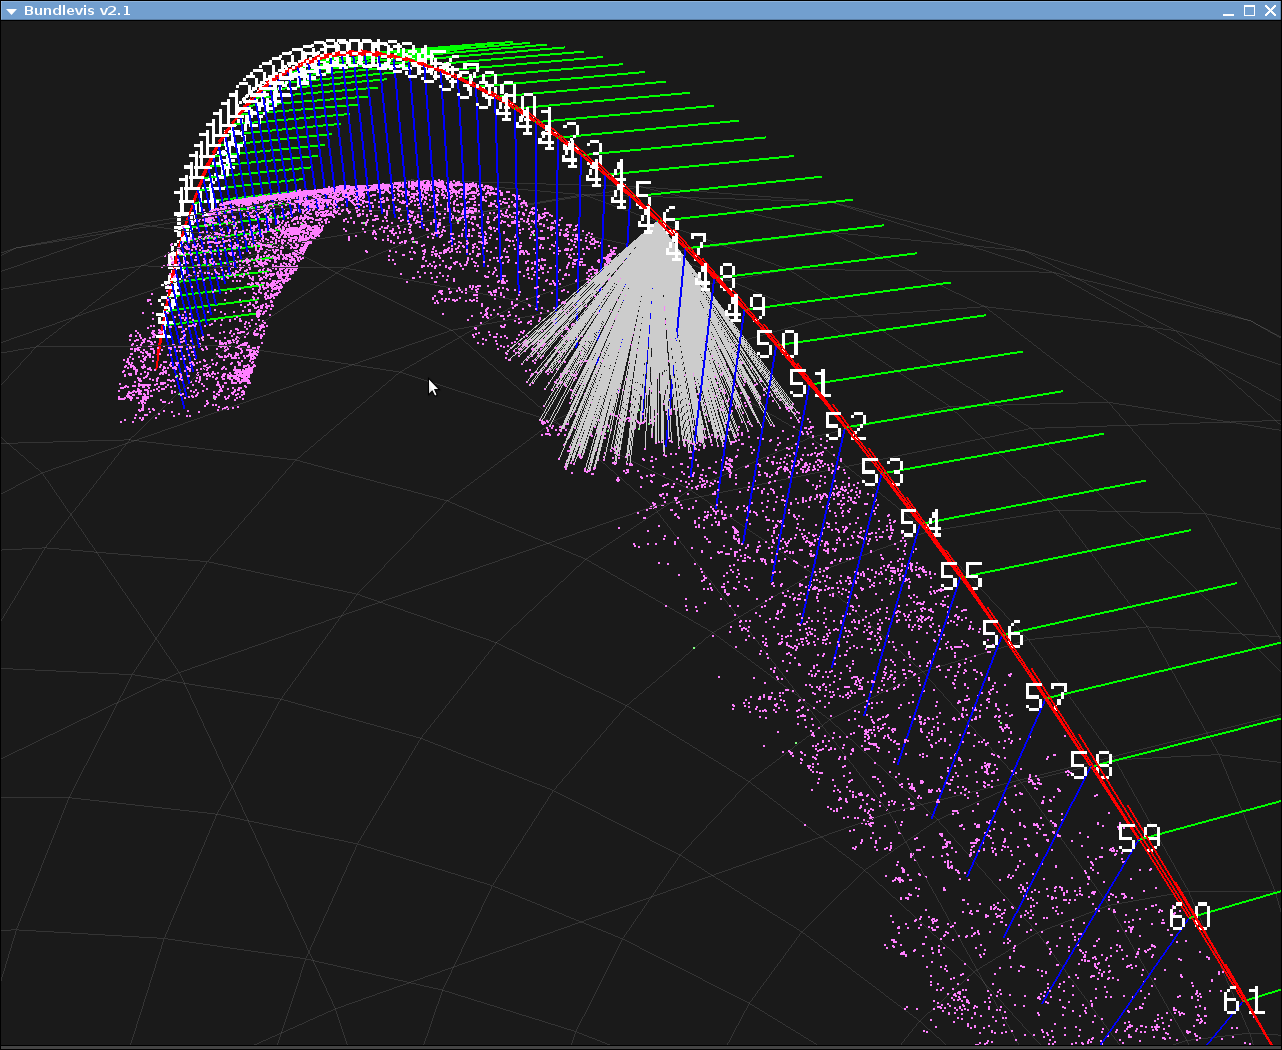
\includegraphics[width=5in]{images/bundlevis_apollo.png}
  \end{center}
  \caption{ A screenshot of bundle adjustment of Apollo 15's Orbit 33. }
  \label{fig:bundlevis}
\end{figure}

After Bundlevis has loaded all the data, the user can inspect the 3D
points that are in purple and play back the iterations. The user is
able to double click on a camera and have lines drawn to each point
viewed by the camera. It also allows the reverse, the user can double
click on a point and have lines drawn to all cameras that view the
point.

Failure of Bundle Adjustment looks different in every case,
but 2 important observations are dead giveaways of a failure. First,
is segmentation, this is different layers developing amoung the
points. This will produce cliffs between the layers and is usually a
sign of poor matching between cameras; specifically the lack of
matches between cameras. The second common sign of a failure is a
point cloud explosion or implosion. This is a sign of poor matching
that has a high number of outliers. In this case it is created
by outlier matches between cameras that physically could not have viewed the
same terrian.


\subsection{Options}

The following is a listing and explanation of the command line options
that can be fed to \texttt{bundlevis} from the terminal.

\begin{verbatim}
--camera-iteration-file, -c [bundlevis camera iteration file]
\end{verbatim}

\emph{Optional.} Only if the camera iteration file is given will
\texttt{bundlevis} draw the cameras used during Bundle Adjustment.

\begin{verbatim}
--points-iteration-file, -p [bundlevis point iteration file]
\end{verbatim}

\emph{Optional.} Likewise, only when giving a point iteration file
will \texttt{bundlevis} draw the ground point estimations used during
Bundle Adjustment.

\begin{verbatim}
--control-network-file, -n [Vision Workbench binary control network file]
\end{verbatim}

\emph{Optional.} When the control network file used during bundle
adjustment is given with the options \verb=--camera-iteration-file=
and \verb=--points-iteration-file=, will \texttt{bundlevis} have the
option to draw the lines that show the relationship between points and
cameras.

\begin{verbatim}
--additional-pnt-files [bundlevis point iteration files]
\end{verbatim}

\emph{Optional.} Additional points can be drawn and animated with the
previously mention data using this option. The files given must be in
the same format as a bundlevis point iteration file and have the same
number of iterations as well.

\begin{verbatim}
--fullscreen
\end{verbatim}

\emph{Optional.} Displays bundlevis using the entire screen, otherwise
the program loads in a window. \emph{It is known that the fullscreen
  option does not work correctly with dual screen systems.}

\begin{verbatim}
--stereo
\end{verbatim}

\emph{Optional.} This forces the program to display in red/blue anaglyph mode.

\begin{verbatim}
--show-moon
\end{verbatim}

\emph{Optional.} Draws a wireframe sphere that represents the Moon.

\begin{verbatim}
--show-mars
\end{verbatim}

\emph{Optional.} Draws a wireframe sphere that represents Mars.

\begin{verbatim}
--show-earth
\end{verbatim}

\emph{Optional.} Draws a wireframe sphere that represents Earth.

\subsection{Controls}

Once \texttt{bundlevis} is running, there are several controls the user can use to interface with the program. There are the playback controls, jump-to-frame controls, and the mouse.

\paragraph{Playback Controls}
Playback controls are similar to winamp, or alternatively described as
being in the same arrangement as the controls on a tape deck.

\newenvironment{myindentpar}[1]
               {\begin{list}{}
                   {\setlength{\leftmargin}{#1}}
                 \item[]
               }
               {\end{list}}

\begin{myindentpar}{3cm}
\begin{description}
  \item[Z] Step back one iteration
  \item[X] Play
  \item[C] Pause
  \item[V] Stop \emph{(which is the same as Pause except that
    bundlevis goes back to iteration 0)}
  \item[B] Step forward one iteration
\end{description}
\end{myindentpar}

\paragraph{Jump-to-Frame Controls}
Jump-to-Frame controls are the numbers \textbf{1-9} along the top of the
keyboard. Pressing \textbf{1} will have \texttt{bundlevis} display the
very first iteration. Pressing \textbf{9} will have \texttt{bundlevis}
display the very last iteration. Pressing \textbf{2} through
\textbf{8} will cause \texttt{bundlevis} to display the iteration that
is somewhere relatively in the middle based on the value of the
number. Finally, there is an option to press \textbf{0} which will
cause \texttt{bundlevis} to display the points at their very last
iteration with an additional tail pointing back to the starting
position of the points in the first iteration.

\paragraph{Mouse}
The mouse is used to move around the model, and has the same controls
as in \texttt{osgviewer}. The \textbf{left mouse button} is rotate,
\textbf{right mouse button} is zoom, and the \textbf{middle mouse
  button} is translation. Alternatively for systems where the mouse is
button challenged, \textbf{option + mouse} is translation and
\textbf{command + mouse} is zoom. Double clicking with the mouse on a
point or camera will allow the user to interact with the model. If the
terminal is still visible, the point number and camera number can be
seen printed after a double click event happens. The final way to
determine what the camera's or point's number is; is to just zoom in
with the mouse. Even all the points will develop numbers above them
once the viewer is within a certain range.

\section{Examples of Use}

\subsection{Processing Mars Orbital Camera}

What follows is an example of using two Mars Orbital Camera (MOC)
images of the south Cydonia region with \texttt{isis\_adjust}. We'll
be using images M10/00254 and R09/01059. These images are available
at Malin Space Science System's website
[\emph{http://www.msss.com/moc\_gallery/}] and at NASA's Planetary
Data System [\emph{http://pds.jpl.nasa.gov/index.shtml}]; be sure to
download the IMQ or IMG format. For reference, the following ISIS commands
are how to convert the MOC images to ISIS cubes.

\begin{verbatim}
        moc2isis from=m1000254.im? to=m1000254.lev0.cub
        moc2isis from=r0901059.im? to=r0901059.lev0.cub

        spiceinit from=m1000254.lev0.cub
        spiceinit from=r0901059.lev0.cub

        moccal from=m1000254.lev0.cub to=m1000254.cub
        moccal from=r0901059.lev0.cub to=r0901059.cub

        rm *.im? *.lev0.cub
\end{verbatim}

At this point a match file needs to be created that connects our to
cube files. Vision Workbench doesn't except cube files. So before
trying to match them; they'll have to be converted to a standard image
format.

\begin{verbatim}
        isis2std from=m1000254.cub to=m1000254.png format=PNG
        isis2std from=r0901059.cub to=r0901059.png format=PNG
\end{verbatim}

Here is how to process those newly created PNG files for interest
points using the tools available in Vision Workbench.

\begin{verbatim}
        ipfind  m1000254.png r0901059.png
        ipmatch m1000254.png r0901059.png -d -r homography
\end{verbatim}

\definecolor{lgray}{gray}{0.95}
\begin{center}
\fcolorbox{black}{lgray}{ \begin{minipage}{5.5in} 

    \emph{Note from Author:} \\ Within IRG it has become apparent that
    using the interest point tools available from Vision Workbench
    does not produces enough matches to continue with Bundle
    Adjustment. The alternative is to use an outside method such as
    SURF \cite{surf09}. The trick is modifing an outside method's
    source code to export a Vision Workbench style match file. This
    can be difficult. Fortunately the patches to do this trick to the
    SURF code is available in the Appendix.  \\ \\ For this example it
    is okay to use the results from \texttt{ipfind} and
    \texttt{ipmatch}. Expect to find approximately 46 matched
    points. Your results will be slightly different due to the random
    nature of RANSAC.
\end{minipage}}
\end{center}

Finally, it is time to start Bundle Adjustment. There are many options
that can be done here. Below shows the options required to create
visualization data for \texttt{bundlevis}, setting the maximium
iterations to 100, and finally the option to create a detailed report
file of \texttt{isis\_adjust}'s results.

\begin{verbatim}
        isis_adjust *.cub -s --max 100 -r 50
\end{verbatim}

The command window should spurt forth a lot of text and the directory
containing this project should suddenly have a lot more files. Don't
panic! This is perfectly normal! Looking through the output in the
terminal or alternatively in the output report file,
\verb=isis_adjust.report=, the problem should have convereged in 35
iterations. The error barely changed, this can be attributed to Mars
Global Surveyor's relative positioning between images being very good. 

Visualizing all the data that was exported for \texttt{bundlevis} is bit of a
long chain of options in the terminal.

\begin{verbatim}
        bundlevis -p iterPointsParam.txt -c iterCameraParam.txt 
                  -n isis_adjust.cnet
\end{verbatim}

Press escape to exit out of \texttt{bundlevis} when
finished. Alternatively we can view a wireframe of Mars as well to
give some perspective. Unforunately this is a bit absurd in this case
since MOC covers such a small area.

\begin{verbatim}
        bundlevis -p iterPointsParam.txt -c iterCameraParam.txt
                  -n isis_adjust.cnet --show-mars
\end{verbatim}

Producing DEMs using the newly created corrections is the same as
covered in Chapter 3. There is one fine difference in that
\texttt{stereo} needs to know of the existence of the correction
files, \verb=m1000254.isis_adjust= and
\verb=r0901059.isis_adjust=. Here is how that is done:

\begin{verbatim}
        stereo m1000254.cub r0901059.cub m1000254.isis_adjust
               r0901059.isis_adjust MOC_RESULTS/M1000254_R0901059
\end{verbatim}

\texttt{stereo} is excepting the correction files in the place where
it would optionally accept a camera model file. It decides what to do
with the input based on the file extension, in this case it is
\verb=.isis_adjust=.

\subsection{Processing with Ground Control Points}

Much like how \texttt{isis\_adjust} will automatically look for match
files in the current working directory to connect it's input files, it
will do the same for ground control points. Ground control point files
are written with the extension \verb=.gcp= and are expected to have
the same name as the image file for which they are paired with.

Below is an example of what is inside a ground control point file
meant for an Apollo Metric Camera image 1125 from Apollo 15's Orbit
33.

\begin{verbatim}
   3305     3811    17.081049  20.173588  1734697.6    100   100   100
   1676.37  926.12  15.638650  24.560510  1734771.35   100   100   100
   3646.08  631.37  18.663032  24.358845  1734745.22   100   100   100
   1206.38  2995.9  14.306318  21.909843  1734746.16   100   100   100
   2872     2154    16.983669  22.560025  1734726.48   100   100   100
\end{verbatim}

First it's important to note that these numbers are not spaced with
actual spaces, but instead there is a tab character between each
column of numbers. Here is what the columns mean:

\begin{myindentpar}{2cm}
\begin{description}
  \item[Column 1:] Sample Number or X location
  \item[Column 2:] Line Number or Y location
  \item[Column 3:] Longitude in degrees
  \item[Column 4:] Latitude in degrees
  \item[Column 5:] Radius in meters
  \item[Column 6-8:] Sigma \emph{(uncertainty)} in meters in the X,Y,
    and Z directions respectively.
\end{description}
\end{myindentpar}

If multiple cameras see the same ground control point, then in each
gcp file at the line containing the shared measurement; make sure they
have the exact same recorded longitude, latitude, and
radius. \texttt{isis\_adjust} will notice this and will make the
connection in the control network.

\subsection{Sharing Data with ISIS3's Qnet}

ISIS contains a program called \texttt{qnet} and it's purpose is to
create and edit ISIS style control network files. To share a control
network with \texttt{qnet} we need to save our control network in the
ISIS format. If bundle adjustment has already been performed once and
if we want to reuse the control network use this command to save an
ISIS style control network:

\begin{verbatim}
        isis_adjust -c isis_adjust.cnet --write *.cub
\end{verbatim}

Otherwise if this is the first time performing bundle adjustment and a
control network does not already exist, use:

\begin{verbatim}
        isis_adjust --write *.cub
\end{verbatim}

There should now be an \verb=isis_adjust.net= file in the project's
directory. It will be quite a bit larger than the other control
network file and it can be read and editted with a text editor. Before
starting \texttt{qnet} there is one additional preperation that must
be performed. \texttt{qnet} requires a text file listing of all the
cubes used by the control network. Here's how to create one.

\begin{verbatim}
        ls *.cub > list_of_cubes.lis
\end{verbatim}

Now it is time to start up \texttt{qnet}. This program does not accept
any command line arguments, so just type \texttt{qnet} in the
terminal. Click File$\rightarrow$Open. It will first ask for the list
of cubes. Refer it to the newly created
\verb=list_of_cubes.lis=. Finally it will ask for the control network,
give it \verb=isis_adjust.net=.

\begin{center}
\fcolorbox{black}{lgray}{ \begin{minipage}{5.5in} 

    \emph{Note from Author:} \\ At this time \texttt{qnet} does not
    work with the Apollo Metric Camera's cube files. When loading the
    text file listing of cubes it will promptly error about invalid
    serial numbers for the listed cube files. (03/11/09)
\end{minipage}}
\end{center}

When finished, save the new control network file. Here's how to use
the new control network in \texttt{isis\_adjust}.

\begin{verbatim}
        isis_adjust -c the_new_control_network.net *.cub
\end{verbatim}

\begin{thebibliography}{1}

\bibitem{hartley04} Hartley, R.I. and Zisserman, A. ``Multiple View Geometry in Computer Vision,''
  Cambridge University Press. 2004. pp 597-627.
\bibitem{moore09} Moore, Wright, Schinstock, and Lewis. ``Comparison of Bundle Adjustment Formulations,''
  presented at ASPRS Annual Conf., Baltimore, Maryland, 2009.
\bibitem{triggs00} Triggs, McLauchlan, Hartley, and Fitzgibbon. ``Bundle Adjustment - A Modern Synthesis,''
  Lecture Notes in Computer Science. Vol. 1883, 298. January 2000
\bibitem{surf09} Bay, Gool, and Tuytelaars. (2009, Mar.). ``SURF: Speeded Up Robust Features'' [Online]. Available: \verb!http://www.vision.ee.ethz.ch/~surf/download.html!

\end{thebibliography}
